\section{Inference and Uncertainty}

\begin{frame} 

\begin{center} \footnotesize
\textit{``As far as the laws of mathematics refer to reality, they are not certain; and as far as they are certain, they do not refer to reality."}
\end{center} 
\begin{flushright} \footnotesize
Albert Einstein, 1921
\end{flushright}

\mode<presentation>{
    \vspace{10mm}
    \begin{center} \huge
        \secname
    \end{center}
    \vspace{10mm}
    }
Because we need to
    \begin{itemize}
    \item[] quantify our degree of belief/\\
	\item[] quantify our uncertainty
    \end{itemize}
    
\end{frame}

\subsection{The probabilistic model}

\begin{frame}\frametitle{\subsecname}

% Please add the following required packages to your document preamble:
% \usepackage{graphicx}
\begin{table}[]
\centering
%\resizebox{\textwidth}{!}{%
\begin{tabular}{rclllllllc}
\multicolumn{1}{c|}{input}                                                         &                                                 &  &  &                       &                                                                                &  &  &  & P($cat$=true)        \\ \cline{1-2} \cline{6-6}
\multicolumn{1}{r|}{\begin{tabular}[c]{@{}r@{}}has\_fur\\ barks\\ meows\end{tabular}} & \multicolumn{1}{c}{\begin{tabular}[c]{@{}c@{}}1\\ 0\\ 1\end{tabular}} &  & $\longrightarrow$ &  & \multicolumn{1}{|c|}{\begin{tabular}[c]{@{}c@{}}model\end{tabular}} &  & $\longrightarrow$ &  & 0.99                 \\ \cline{6-6}
\end{tabular}%
%}
\end{table}

\end{frame}

\begin{frame}\frametitle{\subsecname}

\slidesonly{\vspace{-3mm}}

\begin{figure}[h]
     \centering
	 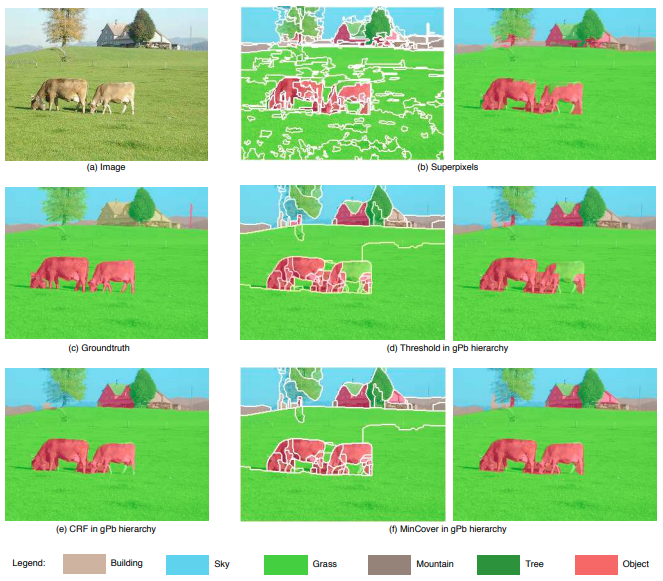
\includegraphics[width=0.7\textwidth]{img/farabet}%
	 \caption{Semantic segmentation (pixel-level classification) \citep{farabet2012learning}}
\end{figure}
\end{frame}

\begin{frame}\frametitle{\subsecname}

\begin{itemize}
    \item \underline{the model:}\\
        \begin{align}
            P(H): H \rightarrow [0,1]&\\
            P(H) = 0 & \quad\iff H \text{ is false (i.e. impossible)} \\
            P(H) = 1 & \quad\iff H \text{ is true (i.e. certain)} \\
            0 < P(H) < 1 & \quad\;\;\text{quantifies our degree of belief}
        \end{align}
    \pause
    
    \mode<presentation>{
    \only<2->{
    \placeimage{11}{9}{img/dice}{width=2cm}
	}
	}
    
    \item \underline{events}: assignment to a set of cases\\
    (e.g. two dice add up to 11)
    \pause
    \item \underline{proposition}: disjunction of \textbf{events}\\
    (i.e. isolate the sets of \textbf{events} in which the \textbf{proposition} holds)\\
    			\iitem{ e.g.~$cavity = \text{true}$ is equivalent to: \\
				{\small
				$(cavity = \text{true} \wedge toothache = \text{false} 
				\wedge catch = \text{false}) \vee$ \\
				$(cavity = \text{true} \wedge toothache = \text{true} 
				\wedge catch = \text{true}) \vee ...$ }
			}
    
\end{itemize}
    
\end{frame}

\begin{frame}

$\underbrace{\text{\emph{Summing over}}}_{\text{marginalisation}}$ the probabilities of the \textbf{events} \\
$\qquad\qquad\qquad\leadsto$ probability of \textbf{proposition}.\\

\pause

Example with dice:

\begin{align}
\overbrace{P({total} = 11)}^{\text{A}} &= \overbrace{P({die}_{1} = 5, {die}_{2} = 6)}^{\text{B}} + \overbrace{P({die}_{1} = 6, {die}_{2} = 5)}^{\text{C}}\\
        %&\stackrel{\text{shorthand}}{=} P(5,6) + P(6,5)\\
        &= 1 / 36 + 1/36\\
        &= 1/18
\end{align}

The terms A,B and C are \emph{unconditional} or \emph{prior} probabilities.\\
They represent the degree of belief in the absence of any other information.\\
Priors are also referred to as \emph{domain knowledge}.
        
\end{frame}

\subsection{Evidence}

\begin{frame}\frametitle{\subsecname}

What if we already \emph{know} (i.e. observed) something?\\

    \mode<presentation>{
    \placeimage{12}{4}{img/dice_obs}{width=2cm}
	}

e.g. We've already rolled the first die and got 5.\\
Now we're waiting to roll the second die.\\

We are now interested in the \emph{conditional} (or \emph{posterior}) probability of the second die leading to a total of 11:

\begin{equation}
P(\;\;{total}= 11 \kern-1.5ex  \underbrace{\big| }_{\text{``given''}} \kern-1.5ex \overbrace{{die}_{1}}^{\mathclap{\{1,2,3,4,5,6\}}} = 5\;\;)
\end{equation}

\end{frame}

\begin{frame}\frametitle{A thing about priors}

The prior is valid even after the outcome.

e.g.\\
\begin{itemize}
 \item[] $P( \kern-1ex \overbrace{cavity}^{\substack{\text{shorthand for}\\{cavity}=\text{true}}} \kern-1ex) = 0.2$
 \item[] $P(cavity | \overbrace{toothache}^{{toothache}=\text{true}}) = 0.6$
 \item[] If we observe that a cavity has actually occurred, we don't have to change our prior on cavities.\\
 However, the prior becomes less useful if we proceed to infer other things.
\end{itemize}


\end{frame}

\begin{frame}\frametitle{A thing about priors}
    
\textbf{Caution}\\
\begin{itemize}
\item[$\times$] Whenever $toothache$=true, then $cavity$ is true with probability of 0.6
\item[\checkmark] Whenever $toothache$=true, \underline{and no other information} is available, then $cavity$ is true with probability of 0.6.
\end{itemize}

\textit{other information}: Diagnosis was \underline{no} cavity. In this case, the probability is no longer 0.6, but:
\begin{equation}
P(cavity \,|\, toothache \wedge diagnosis_{cavity} = \text{false}) = 0
\end{equation}

\end{frame}

\begin{frame}\frametitle{We were talking about evidence}

Observing event $e$ rules out events where $e$ is false. This leaves a set where $P(e)>0$.\\
Therefore, when we query for some variable $x$,
we look within that set for the fraction that satisfies $x$ and $e$.

This fraction can be calculated using the following:

\begin{equation}
P(x|e) = \frac{P(x,e)}{P(e)}
\end{equation}

which brings us to the \emph{product rule}:

\begin{equation}
P(x,e) = P(x|e) P(e)
\label{eq:productrule}    
\end{equation}

\end{frame}

\begin{frame}

\question{What information do I need to calculate the probability of any proposition?}

- The full joint probability distribution\notesonly{ provides all the information to calculate the probability of any proposition.}

Example of a full joint distribution between $Cavity,Toothache$ and $Catch$:\\

%\footnotesize
	%\begin{center}
     \begin{table}[h] 
\resizebox{\textwidth}{!}{%
	\begin{tabular}{|c|c|c|}
		\hline
		& $toothache = \text{true}$ & $toothache = \text{false}$ \\
		\begin{tabular}{c}
			\\ 
			$cavity = \text{true}$ \\
			$cavity = \text{false}$
		\end{tabular} 
		& 
		\begin{tabular}{c|c}
			$catch = \text{true}$ & $catch = \text{false}$\\ 
			\hline 
			$0.108$ & $0.012$ \\
			$0.016$ & $0.064$
		\end{tabular} 
		& 
		\begin{tabular}{c|c}
			$catch = \text{true}$ & $catch = \text{false}$\\ 
			\hline 
			$0.072$ & $0.008$ \\
			$0.144$ & $0.576$
		\end{tabular} 
		\\ \hline
	\end{tabular}
	}
    \end{table}
	

\end{frame}

\subsubsection{Marginalisation (``summing out'')}



\begin{frame}\frametitle{\subsubsecname}

\begin{equation}
P(x | \vec e)
= \frac{P(x, \vec e)}{P(\vec e)}
= \alpha P(x, \vec e)
= \alpha \sum_{\vec y \in \vec Y} P(\vec x, \vec e, \vec y)
\end{equation}

where
\begin{itemize}
\item[] $x$: query variable
\item[] $\vec e$: evidence variable(s)
\item[] $\vec y$: \textbf{un}observed variables in the table
\item[] $\alpha$: normalization factor:

\question{How do we calculate the normalization factor $\alpha$?}

\pause

\notesonly{- Via:}
\begin{enumerate}
\item evidence prior:
\begin{equation}
\frac{1}{\alpha} := P(\vec e) = \sum_{x, \vec y} P(x, \vec e, \vec y)  
\end{equation}
\item or simply whatever ensures $\sum_{ x} P(x, \vec e) = 1$
\end{enumerate}

\end{itemize}
    
\end{frame}

\subsubsection{Applying the product rule}

\begin{frame}\frametitle{\subsubsecname}
    
\mode<presentation>{

     \begin{table}[h] 
\resizebox{\textwidth}{!}{%
	\begin{tabular}{|c|c|c|}
		\hline
		& $toothache = \text{true}$ & $toothache = \text{false}$ \\
		\begin{tabular}{c}
			\\ 
			$cavity = \text{true}$ \\
			$cavity = \text{false}$
		\end{tabular} 
		& 
		\begin{tabular}{c|c}
			$catch = \text{true}$ & $catch = \text{false}$\\ 
			\hline 
			$0.108$ & $0.012$ \\
			$0.016$ & $0.064$
		\end{tabular} 
		& 
		\begin{tabular}{c|c}
			$catch = \text{true}$ & $catch = \text{false}$\\ 
			\hline 
			$0.072$ & $0.008$ \\
			$0.144$ & $0.576$
		\end{tabular} 
		\\ \hline
	\end{tabular}
	}
    \end{table}
}

\begin{align}
P(cavity | toothache=\text{true}) \only<1>{&= \frac{P(cavity,toothache)}{P(toothache)}\\
&= \frac{0.108 + 0.012}{0.108 + 0.012 + 0.016 + 0.064}\\}
&= 0.6   
\end{align}

\pause


\begin{equation*}
P(cavity=\text{false} | toothache=\text{true}) = ?
\end{equation*}

\question{What should we expect?}

\pause

\slidesonly{\vspace{-7mm}}

\begin{align}
P(cavity=\text{false} | toothache=\text{true}) &= \frac{P(cavity=\text{false},toothache)}{P(toothache)}\\
&= \frac{0.016 + 0.0064}{0.108 + 0.012 + 0.016 + 0.064}\\
&= 0.4 = 1 - 0.6   
\end{align}

\end{frame}

\begin{frame}


\mode<presentation>{

     \begin{table}[h] 
\resizebox{\textwidth}{!}{%
	\begin{tabular}{|c|c|c|}
		\hline
		& $toothache = \text{true}$ & $toothache = \text{false}$ \\
		\begin{tabular}{c}
			\\ 
			$cavity = \text{true}$ \\
			$cavity = \text{false}$
		\end{tabular} 
		& 
		\begin{tabular}{c|c}
			$catch = \text{true}$ & $catch = \text{false}$\\ 
			\hline 
			$0.108$ & $0.012$ \\
			$0.016$ & $0.064$
		\end{tabular} 
		& 
		\begin{tabular}{c|c}
			$catch = \text{true}$ & $catch = \text{false}$\\ 
			\hline 
			$0.072$ & $0.008$ \\
			$0.144$ & $0.576$
		\end{tabular} 
		\\ \hline
	\end{tabular}
	}
    \end{table}
}

\mode<presentation>{
\only<1>{
\begin{align}
P(cavity=\text{false} | toothache=\text{true}) &= \frac{P(cavity=\text{false},toothache)}{P(toothache)}\\
&= \frac{0.016 + 0.0064}{0.108 + 0.012 + 0.016 + 0.064}\\
&= 0.4 = 1 - 0.6   
\end{align}

\textbf{Remark}: The denominator remains constant no matter which value of cavity we are interested in.\\
$\Rightarrow$ use $1/P(toothache)$ as the normalization factor for $P(Cavity | toothache)$.
}
}

\only<2>{\slidesonly{
\begingroup
\footnotesize
}
\begin{align}
P(\kern-4ex\overbrace{Cavity}^{\footnotesize\rmat{cavity=\text{true}\\cavity=\text{false}}} \kern-4ex |toothache) &= \alpha P(Cavity, toothache) \\
&= \alpha \big\lbrack
P(Cavity, toothache, catch) \\
&\qquad+ P(Cavity, toothache, catch=\text{false}) 
\big\rbrack\\
&= \alpha \bigg\lbrack
\rmat{0.108\\0.016} + \rmat{0.012\\0.064}
\bigg\rbrack\\
&= \alpha \rmat{0.12\\0.08} \stackrel{\substack{\alpha=\\1/P(toothache)}}{=} \rmat{0.6\\0.4}
\intertext{OR normalize s.t. $\sum_{\vec x} P(x, \vec e) \eqexcl 1$}
&= \alpha \rmat{0.12\\0.08} \stackrel{\alpha=\frac{1}{0.12+0.08}}{=} \rmat{0.6\\0.4}
\end{align}\slidesonly{
\endgroup
}
}



\end{frame}
